
\documentclass[10pt]{article}
\usepackage[a4paper, tmargin=0.75in, lmargin=0.80in, rmargin=0.80in, bmargin=1in]{geometry}
\usepackage{hyperref}
\usepackage{dsfont}
\usepackage{amsfonts}
\usepackage{ragged2e}
\usepackage{mathtools}
\usepackage{enumitem}   
\usepackage{MnSymbol}%
\usepackage{wasysym}%
\usepackage{relsize}%
\usepackage{xcolor}

\usepackage{amsmath}
\usepackage{upgreek}
\usepackage{mathrsfs}
\usepackage{blindtext}
\usepackage{listings}
\usepackage{xcolor}


%New colors defined below
\definecolor{codegreen}{rgb}{0,0.6,0}
\definecolor{codegray}{rgb}{0.5,0.5,0.5}
\definecolor{codepurple}{rgb}{0.58,0,0.82}
\definecolor{backcolour}{rgb}{0.95,0.95,0.92}

\lstset{
    literate={ĉ}{{\^c}}1
        {Ĉ}{{\^C}}1
}

%Code listing style named "mystyle"
\lstdefinestyle{mystyle}{
  backgroundcolor=\color{backcolour}, commentstyle=\color{codegreen},
  keywordstyle=\color{magenta},
  numberstyle=\tiny\color{codegray},
  stringstyle=\color{codepurple},
  basicstyle=\ttfamily\footnotesize,
  breakatwhitespace=false,         
  breaklines=true,                 
  captionpos=b,                    
  keepspaces=true,                 
  numbers=left,                    
  numbersep=5pt,                  
  showspaces=false,                
  showstringspaces=false,
  showtabs=false,                  
  tabsize=2
}

\lstset{style=mystyle}


\usepackage{natbib}
\usepackage{graphicx}
\pagestyle{empty}
\renewcommand\thesubsection{\Alph{subsection}}
\DeclareMathOperator*{\limop}{\lim}




%%%%%%%%%%%%%%%%%%%%%%%%%%%%%%%%%%%%%%%%%%%%%%%%%%
%%%%%%%%%%%%%%%%%%%%%%%%%%%%%%%%%%%%%%%%%%%%%%%%%%
%%%%%%%%%%%%%%%%%%%%%%%%%%%%%%%%%%%%%%%%%%%%%%%%%%
%%%%%%%%%%%%%%%%%%%%%%%%%%%%%%%%%%%%%%%%%%%%%%%%%%
% ENTER SOME IMPORTANT INFORMATION
%%%%%%%%%%%%%%%%%%%%%%%%%%%%%%%%%%%%%%%%%%%%%%%%%%
%%%%%%%%%%%%%%%%%%%%%%%%%%%%%%%%%%%%%%%%%%%%%%%%%%
%%%%%%%%%%%%%%%%%%%%%%%%%%%%%%%%%%%%%%%%%%%%%%%%%%
%%%%%%%%%%%%%%%%%%%%%%%%%%%%%%%%%%%%%%%%%%%%%%%%%%
\newcommand{\studentname}{Luis Alejandro Rubiano}
\newcommand{\studentnumber}{202013482}
\newcommand{\researchcentre}{la.rubiano@uniandes.edu.co}
\newcommand{\projecttitle}{Convex Optimization}
\newcommand{\supervisor}{Mauricio Junca}
\newcommand{\xRightarroww}[2][]{\ext@arrow 0359\Rightarrowfill@{#1}{#2}}

\newcommand\setItemnumber[1]{\setcounter{enum\romannumeral\@enumdepth}{\numexpr#1-1\relax}}

\newcommand\restr[2]{{% we make the whole thing an ordinary symbol
  \left.\kern-\nulldelimiterspace % automatically resize the bar with \right
  #1 % the function
  \littletaller % pretend it's a little taller at normal size
  \right|_{#2} % this is the delimiter
  }}

\newcommand{\littletaller}{\mathchoice{\vphantom{\big|}}{}{}{}}


%%%%%%%%%%%%%%%%%%%%%%%%%%%%%%%%%%%%%%%%%%%%%%%%%%
%%%%%%%%%%%%%%%%%%%%%%%%%%%%%%%%%%%%%%%%%%%%%%%%%%
%%%%%%%%%%%%%%%%%%%%%%%%%%%%%%%%%%%%%%%%%%%%%%%%%%
%%%%%%%%%%%%%%%%%%%%%%%%%%%%%%%%%%%%%%%%%%%%%%%%%%
%%%%%%%%%%%%%%%%%%%%%%%%%%%%%%%%%%%%%%%%%%%%%%%%%%
%%%%%%%%%%%%%%%%%%%%%%%%%%%%%%%%%%%%%%%%%%%%%%%%%%

\begin{document}

\begin{center}
{\Huge{Homework 4, Convex Optimization}} \\
\vspace{2mm}
{\Large{Departamento de Matemáticas, Universidad de los Andes}} \\
\vspace{1mm}
{\Large{Colombia}}
\end{center}

\vspace{5mm}
\hrule
\vspace{1mm}
\hrule

\vspace{3mm}
\begin{tabular}{ll} 
Student's name:           	        & {\studentname}   \\ 
Student's code: 	        & {\studentnumber} \\ 
Email address: 	        & {\researchcentre}  \\ 
Class: 	& {\projecttitle}  \\ 
Instructor: 	    & {\supervisor}  \\ 
\end{tabular}

\vspace{3mm}
\hrule
\vspace{1mm}
\hrule

\hfill \break %SPACE

\section{Given $x \in C$ with $C$ a convex set, let $N_C(x) := \{ g : \langle g, y - x \rangle \leq 0, \forall y \in C \}$. }

\begin{enumerate}[label=(\alph*)]
  \item Show that $N_C(x)$ is a closed convex cone.
\end{enumerate}

\paragraph{Proof:}

Let $g_1, g_2 \in N_c(x)$ and $t >0$. Then, 

\begin{align*}
  \langle t g_1, y - x \rangle &= t \langle g_1, y - x \rangle \text{ for all } y \in C\\
  t \langle g_1, y - x \rangle &\leq 0 \text{ since } g_1 \in N_C(x) \text{ and } t > 0\\
\end{align*}

Therefore, $t g_1 \in N_C(x)$. Also, 

\begin{align*}
  \langle g_1 + g_2, y - x \rangle &= \langle g_1, y - x \rangle + \langle g_2, y - x \rangle \text{ for all } y \in C\\
  \langle g_1, y - x \rangle &\leq 0 \text{ since } g_1 \in N_C(x)\\
  \langle g_2, y - x \rangle &\leq 0 \text{ since } g_2 \in N_C(x)\\
  \langle g_1, y - x \rangle + \langle g_2, y - x \rangle &\leq 0\\
\end{align*}

Therefore, $g_1 + g_2 \in N_C(x)$. Thus, $N_C(x)$ is a convex cone.\\

Finally, let $g_n$ be a sequence in $N_C(x)$ that converges to $g$. Since for each 
$g_n \in N_C(x)$, we have that $\langle g_n, y - x \rangle \leq 0$ for all $y \in C$, 
then $$\lim_{n \to \infty} \langle g_n, y - x \rangle \leq 0$$ for all $y \in C$. Because
of the continuity of the inner product, we have that $N_C(x)$ is closed.\\

Hence, $N_C(x)$ is a closed convex cone. $\square$


\hfill \break %SPACE


\begin{enumerate}[label=(\alph*)]
  \setcounter{enumi}{1}
  \item Show that if $x \in \text{int}(C)$, then $N_C(x) = \{0\}$.
\end{enumerate}

\paragraph{Proof:}


Let $x \in \text{int}(C)$, then there is some 
$\varepsilon>0$ such that $B(x, \varepsilon) \subseteq C$. Consider the point 
$y:=x + \varepsilon g$ . Since $x \in \text{int}(C)$, then $y \in C$. 
Then, 

\begin{align*}
  \langle g, y - x \rangle &= \langle g, (x + \varepsilon g) - x \rangle\\
  &= \langle g, \varepsilon g \rangle\\
  &= \varepsilon \| g \|^2 \\
\end{align*}

Since $\varepsilon > 0$, then $g$ must be the zero vector. Therefore, $N_C(x) = \{0\}$. $\square$




\hfill \break %SPACE

\begin{enumerate}[label=(\alph*)]
  \setcounter{enumi}{2}
  \item Find the set for all the points of a closed line segment in $\mathbb{R}^2$.
\end{enumerate}

\paragraph{Solution:}

Line segments in $\mathbb{R}^2$ have one of the following forms:

\begin{enumerate}
  \item Case 1: $C_1 = \{ (x,y): x \in [x_0, x_1], y = m x + b \}$, $m, b, x_0, x_1 \in \mathbb{R}$, $x_0 < x_1$,
  \item Case 2: $C_2 = \{ (x,y): x \in (x_0, x_1), y = m x + b \}$, $m, b, x_0, x_1 \in \mathbb{R}$, $x_0 < x_1$,
  \item Case 3: $C_3 = \{ (x,y): x=c, y \in [y_0, y_1] \}$, $c, y_0, y_1 \in \mathbb{R}$, $y_0 < y_1$,
  \item Case 4: $C_4 = \{ (x,y): x=c, y \in (y_0, y_1) \}$, $c, y_0, y_1 \in \mathbb{R}$. $y_0 < y_1$.
\end{enumerate}

We will go through each case:

\begin{enumerate}
  \item Case 1: 
\end{enumerate}

Let $z = (z_x, z_y) \in C_1$. If $z_x \in (x_0, x_1)$, then $N_{C_1}(z) = \{ 0 \}$ because of (b).
If $z = (x_0, m x_0 + b)$, then 

\begin{align*}
  N_{C_1}(z) &= \{ g: \langle g, r - z \rangle \leq 0, \forall r \in C_1 \}\\
  &= \{ g: g_x (r_0 - x_0) + g_y ((m r_0 + b) - (m x_0 + b)) \leq 0, \forall r_0 \in [x_0, x_1] \}\\
  &= \{ g: g_x (r_0 - x_0) + g_y (m (r_0 - x_0)) \leq 0, \forall r_0 \in [x_0, x_1] \}\\
  &= \{ g: g_x + m g_y \leq 0\} \text{ since $r_0 - x_0 \geq 0$}\\
\end{align*}

If $z = (x_1, m x_1 + b)$, then

\begin{align*}
  N_{C_1}(z) &= \{ g: \langle g, r - z \rangle \leq 0, \forall r \in C_1 \}\\
  &= \{ g: g_x (r_1 - x_1) + g_y ((m r_1 + b) - (m x_1 + b)) \leq 0, \forall r_1 \in [x_0, x_1] \}\\
  &= \{ g: g_x (r_1 - x_1) + g_y (m (r_1 - x_1)) \leq 0, \forall r_1 \in [x_0, x_1] \}\\
  &= \{ g: g_x + m g_y \geq 0\} \text{ since $r_0 - x_0 \leq 0$}\\
\end{align*}


\begin{enumerate}
  \setcounter{enumi}{1}
  \item Case 2:
\end{enumerate}

In this case $N_{C_2}(z) = \{ 0 \}$ for all $z \in C_2$ because of (b).\\

\begin{enumerate}
  \setcounter{enumi}{2}
  \item Case 3:
\end{enumerate}

Let $z = (z_x, z_y) \in C_3$. If $z_y \in (y_0, y_1)$, then $N_{C_3}(z) = \{ 0 \}$ because of (b).
If $z = (c, y_0)$, then 

\begin{align*}
  N_{C_3}(z) &= \{ g: \langle g, r - z \rangle \leq 0, \forall r \in C_3 \}\\
  &= \{ g: g_x (c - c) + g_y (r_y - y_0) \leq 0, \forall r_y \in [y_0, y_1] \}\\
  &= \{ g: g_y \leq 0\} \text{ since } r_y - y_0 \geq 0 \\
\end{align*}

Likewise, if $z = (c, y_1)$, then $N_{C_3}(z) = \{ g: g_y \geq 0\}$.\\

\begin{enumerate}
  \setcounter{enumi}{3}
  \item Case 4:
\end{enumerate}

In this case $N_{C_4}(z) = \{ 0 \}$ for all $z \in C_4$ because of (b). $\square$




\hfill \break %SPACE


\section{\textit{Convex hull or envelope of a function. } The convex hull 
or envelope of a function $f: \mathbb{R}^n \rightarrow \mathbb{R}$ is defined as
$$g(x) = \inf\{ t \ | \ (x,t) \in \textbf{conv epi } f \}$$
Geometrically, the epigraph of $g$ is the convex hull of the epigraph of $f$.
Show that $g$ is the largest convex underestimator of $f$. In other words, show that if $h$ is convex and 
satisfies $h(x) \leq f(x)$ for all $x$, then $h(x)\leq g(x)$ for all $x$. Ex. 3.30. Convex Optimization, Boyd.}

\paragraph{Solution:}

Let $h$ be a convex function such that $h(x) \leq f(x)$ for all $x$. 
Since $h$ is convex, $\textbf{epi } h$ is a convex set. Since $h(x) \leq f(x)$ for all $x$, then
$\textbf{epi } f \subseteq \textbf{epi } h$. Therefore, $\textbf{conv epi } f = \textbf{epi } g \subseteq \textbf{epi } h$.
Or equivalently, $g(x) \leq h(x)$ for all $x$. This is because the convex hull of $\textbf{epi } f$ is the intersection 
of all convex sets that contain $\textbf{epi } f$. $\square$
 
\hfill \break %SPACE

\setcounter{section}{3}

\section{Consider the function $f(x)=\langle c, x \rangle - \sum_{j=1}^m \log(1- \langle a_j, x \rangle) - \sum_{i=1}^n \log(1 - x_i^2)$. Take $n=5000$ and $m=2000$ 
and vectors $c$ and $a_j$ chocen arbitrarily such that $\| a_j \| = 1$. For all methods start the iterations at $x_0 = 0$ and 
stopping criterion $\| \nabla f(x_k) \| \leq \varepsilon$. Graph $\log(f(x_k) - f^*)$ in each iteration (estimate $f^*$ as best as possible)
and compare the execution time of the methods.}

\begin{enumerate}
  \item Use the quasi-Newton BFGS method with \textit{backtracking} and Wolfe to chose the step size. Graph the condition number of $H_k$ in each iteration.
\end{enumerate}

\paragraph{Solution:}

This method took $3.79$ hours to complete. Python3 code to solve this problem is given by:


\begin{lstlisting}[language=Python]
import matplotlib.pyplot as plt
import os
from time import perf_counter
from numpy import float16, dot, ones, zeros, identity, log, outer, sqrt
from numpy.linalg import norm, solve, cond
import pandas as pd
from progress.bar import Bar
from random import sample

n = 5000
m = 2000
epsilon = float16(1e-6)
# C is the vector of ones
ONE = float16(1)
TWO = float16(2)
rho = float16(0.75)

f_optimal = -1264.24311

max_iterations = 20 # Maximum number of iterations
max_sub_iterations = 5 # Maximum number of sub-iterations

dots = {}
def optimized_dot(x,y):
    stringxy = str(x) + str(y)
    if stringxy in dots:
        return dots[stringxy]
    result = dot(x,y)
    dots[stringxy] = result
    return result

fs = {}
def f(x, A):
    stringx = str(x)
    if stringx in fs:
        return fs[stringx]

    result = sum(x)
    for j in range(m):
        result -= log(ONE - optimized_dot(A[j],x))
    for i in range(n):
        result -= log(ONE - x[i]*x[i])

    fs[stringx] = result
    return result

gradients = {}
def gradient(x, A):
    stringx = str(x)
    if stringx in gradients:
        return gradients[stringx]

    result = ones(n)
    with Bar('Gradient', fill='#', suffix='%(percent).1f%% - %(eta)ds', max=n) as bar:
        for i in range(n):
            for j in range(m):
                result[i] += A[j][i] / (ONE - optimized_dot(A[j],x))
            result[i] += TWO * x[i] / (ONE - x[i]*x[i])
            bar.next()

    gradients[stringx] = result
    return result

def graph(x, y, title, x_label, y_label, filename):
    fig = plt.figure()
    plt.plot(x, y)
    plt.title(title)
    plt.xlabel(x_label)
    plt.gca().xaxis.set_major_locator(plt.MaxNLocator(integer=True))
    plt.ylabel(y_label)
    filename = "images" + os.sep + filename + ".png"
    fig.savefig(filename, dpi=fig.dpi)
    plt.clf()

A = []
df = pd.read_csv('A.txt', header=None)
data = df.values
for j in range(m):
    # Save data[j] as numpy array of float16
    A.append(data[j].astype(float16))
print("A loaded")

## quasi-Newton BFGS with backtracking and wolfe conditions

time0 = perf_counter()


alpha = float16(0.15) # Initial alpha
c_1 = float16(10e-4)
c_2 = float16(0.9)
X = [zeros(n, dtype=float16)] # Initial point x_0 = 0
Fx = [f(X[-1],A)]
GRADIENTS = [gradient(X[-1], A)]
ALPHAS = [alpha]
H = [identity(n)]
P = [-H[-1] @ GRADIENTS[-1]]
H_condition_numbers = [cond(H[-1])]

iterations = 0


while (norm(GRADIENTS[-1]) > epsilon) and (iterations < max_iterations):
    print("Iteration", iterations)
    print("Condition number of H_k:", H_condition_numbers[-1])
    print("f(x_k):", Fx[-1])
    print("x_k:", X[-1]) 

    iterations += 1
    sub_iterations = 0
    
    while (f(X[-1] + ALPHAS[-1] * P[-1], A) > f(X[-1], A) + c_1 * ALPHAS[-1] * optimized_dot(gradient(X[-1], A), P[-1]) 
           or (- optimized_dot(gradient(X[-1] + ALPHAS[-1] * P[-1], A), P[-1]) > - c_2 * optimized_dot(gradient(X[-1], A), P[-1]))
           ) and sub_iterations < max_sub_iterations:
        sub_iterations += 1
        ALPHAS[-1] = rho * ALPHAS[-1]

    X.append(X[-1] + ALPHAS[-1] * P[-1]) # X_k+1 = X_k + alpha * P_k
    Fx.append(f(X[-1], A))
    GRADIENTS.append(gradient(X[-1], A))
    s = X[-1] - X[-2]
    y = GRADIENTS[-1] - GRADIENTS[-2]
    ALPHAS.append(alpha)
    H.append(H[-1] - (H[-1]@ (outer(y,y) @H[-1]))/(y.T @(H[-1]@y)) + outer(s,s)/(optimized_dot(y,s)))
    P.append(- H[-1] @ GRADIENTS[-1])
    H_condition_numbers.append(cond(H[-1]))

time1 = perf_counter()

print("Quasi-Newton BFGS with backtracking and wolfe conditions completed")
print("Iterations:", iterations)
print("Total time elapsed:", (time1 - time0)/3600, "hours")

log_Fx = [log(f - f_optimal) for f in Fx]
graph(range(iterations+1), log_Fx, "log(f(x)-f*) vs iterations", "Iteration", "log(f(x)-f*)", "4ai")
graph(range(iterations+1), H_condition_numbers, "Condition number of H vs iterations", "Iteration", "Condition number of H", "4aii")

\end{lstlisting}

\begin{figure}[!tbp]
  \centering
  \begin{minipage}[b]{0.4\textwidth}
      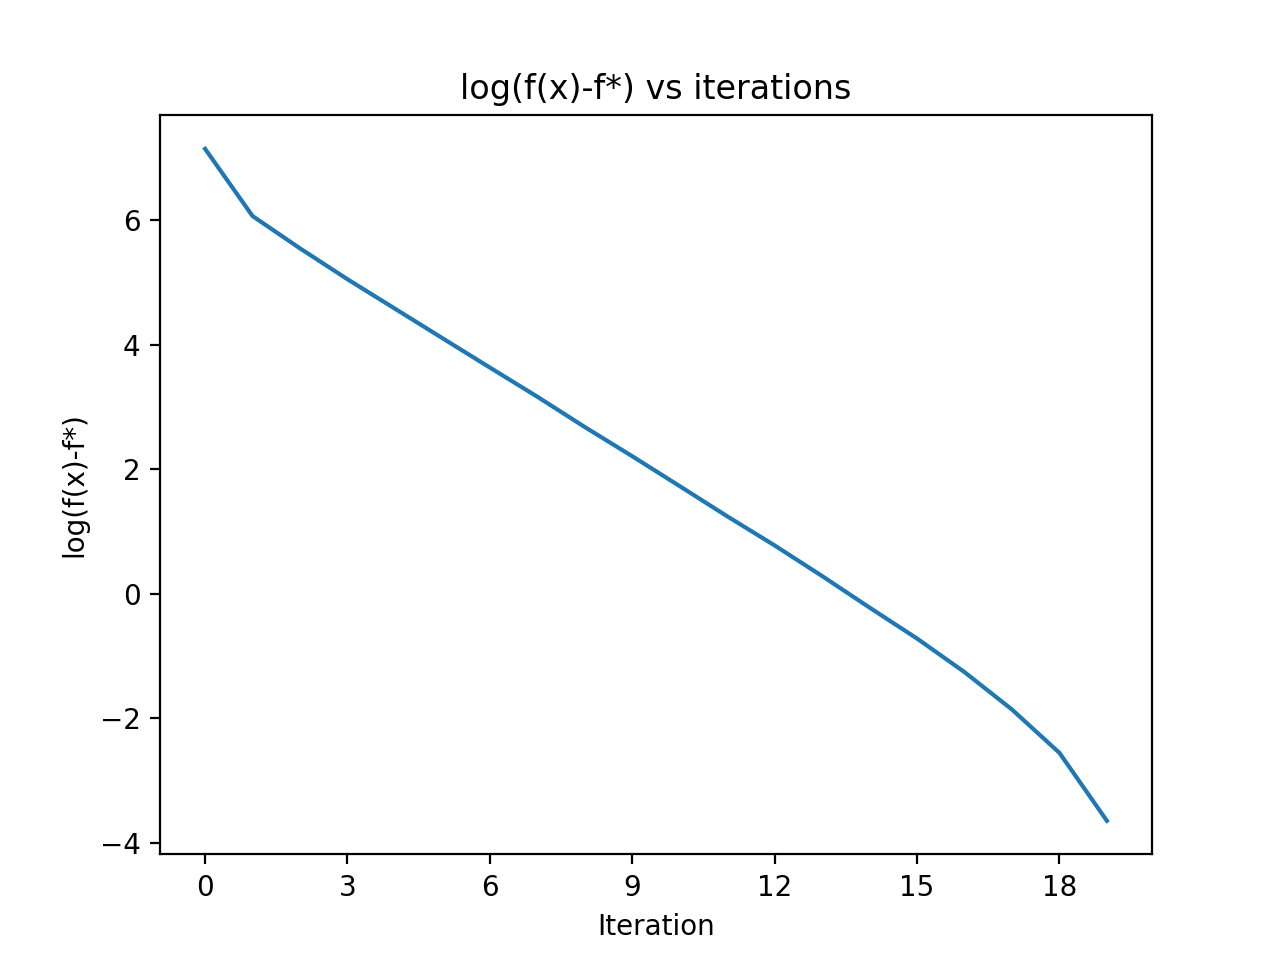
\includegraphics[width=\textwidth]{images/4ai.png}
      \caption{$\log(f(x) - f^*)$, using quasi-Newton BFGS method, $x_0 = 0$}
  \end{minipage}
  \hfill
  \begin{minipage}[b]{0.4\textwidth}
      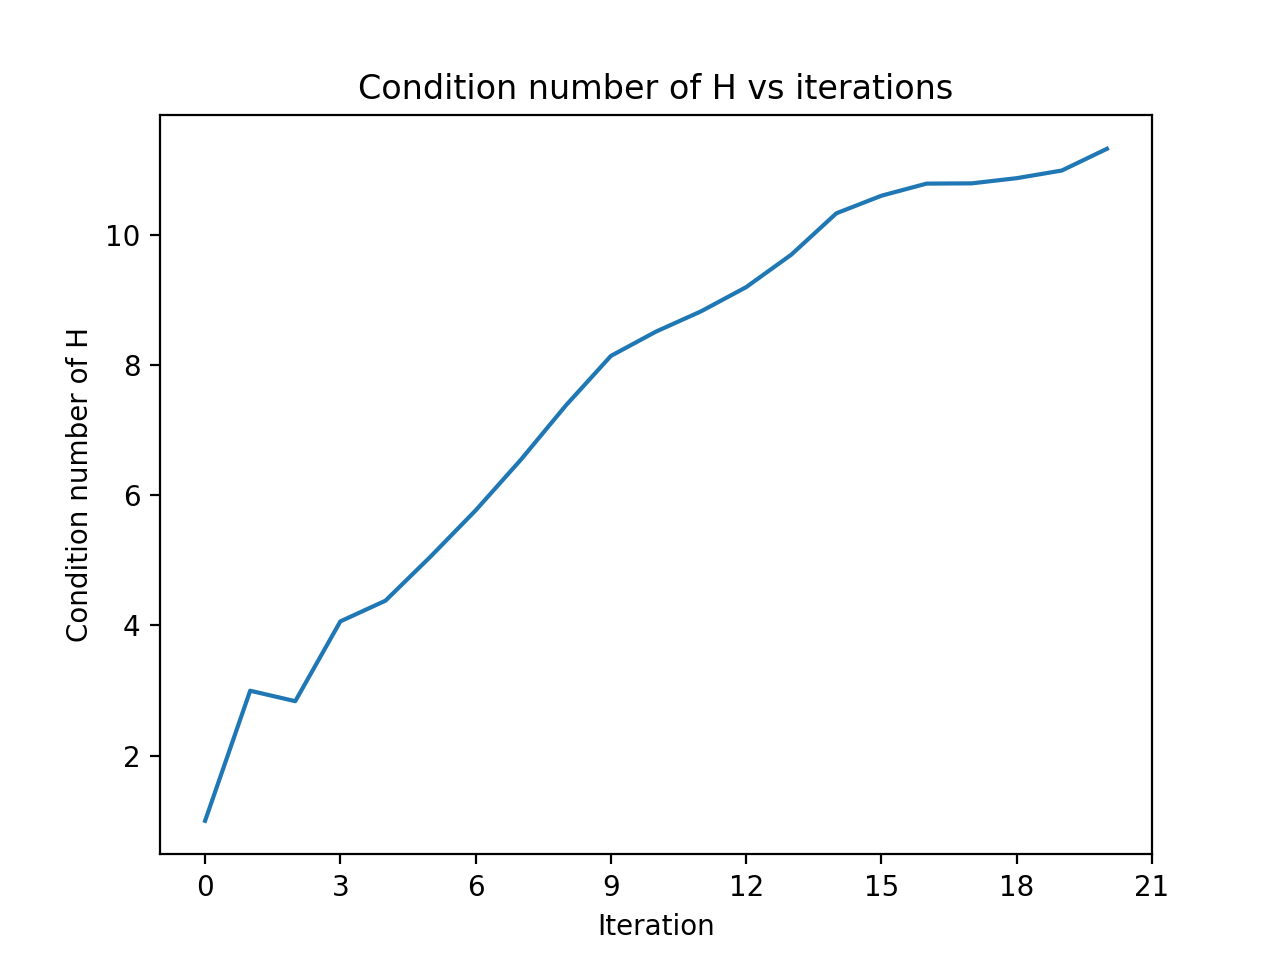
\includegraphics[width=\textwidth]{images/4aii.png}
      \caption{Condition number of $H_k$, using quasi-Newton BFGS method, $x_0 = 0$}
  \end{minipage}

\end{figure}

\hfill \break %SPACE





\begin{enumerate}
  \setcounter{enumi}{1}
  \item Use the confidence region Newton method and the \textit{dogleg} method to approximate solution to the subproblem. Graph $\Delta_k$ in each iteration.
\end{enumerate}

\paragraph{Solution:}



This method took $3.61$ hours to complete. Python3 code to solve this problem is given by:


\begin{lstlisting}[language=Python]
  ## Confidence region Newton method 

  dots = {}
  fs = {}
  gradients = {}
  zero_vector = zeros(n)
  
  def dogleg(grad, hess, rad):
      p_B = -solve(hess, grad)
      p_U = - optimized_dot(grad, grad) / (grad.T @ hess @ grad) * grad
  
      if norm(p_B) <= rad:
          return p_B
      elif norm(p_U) >= rad:
          return rad/norm(p_U) * p_U
      else:
          a = optimized_dot(p_B, p_B) - 2 * optimized_dot(p_B, p_U) + optimized_dot(p_U, p_U)
          b = 2 * optimized_dot(p_B, p_U) - 2 * optimized_dot(p_U, p_U)
          c = optimized_dot(p_U, p_U) - rad**2
          tau_minus_one = (-b + (b**2 - 4*a*c)**0.5) / (2*a)
          return p_U + tau_minus_one * (p_B - p_U)
      
  def m_function_generator(fx, hess, grad):
      return lambda p: fx + optimized_dot(grad, p) + 0.5 * p.T @ hess @ p
  
          
  def compute_rho(f, x, p, A, m):
      return (f(x, A) - f(x + p, A)) / (m(zero_vector)-m(p))
  
  
  time2 = perf_counter()
  X = [zeros(n, dtype=float16)] # Initial point x_0 = 0
  Fx = [f(X[-1],A)]
  DELTAS = [0.05] # Radius of the confidence region
  Delta_max = 0.25
  H = [identity(n)] # Initial Hessian
  GRADIENTS = [gradient(X[-1], A)] # Initial gradient
  eta = 0.25 # threshold
  P = [dogleg(GRADIENTS[-1], H[-1], DELTAS[-1])] # Initial step
  M = [m_function_generator(f(X[-1], A), H[-1], GRADIENTS[-1])] # Initial m function
  Rho = [compute_rho(f, X[-1], P[-1], A, M[-1])] # Initial rho
  
  iterations = 0
  
  while (norm(GRADIENTS[-1]) > epsilon) and (iterations < max_iterations):
      print("Iteration", iterations)
      print("f(x_k):", f(X[-1],A))
      print("x_k:", X[-1]) 
      print("Delta_k:", DELTAS[-1])
  
      iterations += 1
      sub_iterations = 0
  
      if Rho[-1] < 0.25:
          DELTAS.append(DELTAS[-1] / 4)
      else:
          if Rho[-1] > 0.75 and norm(P[-1]) == DELTAS[-1]:
              DELTAS.append(min(2*DELTAS[-1], Delta_max))
          else:
              DELTAS.append(DELTAS[-1])
      
      if Rho[-1] > eta:
          X.append(X[-1] + P[-1])
      else:
          X.append(X[-1]) 
  
      # Delta and X were updated, now we update the other
  
      Fx.append(f(X[-1], A))
      GRADIENTS.append(gradient(X[-1], A))
  
      s = X[-1] - X[-2] #Update H by BFGS formula
      y = GRADIENTS[-1] - GRADIENTS[-2]
      H.append(H[-1] - (H[-1]@ (outer(y,y) @H[-1]))/(y.T @(H[-1]@y)) + outer(s,s)/(optimized_dot(y,s)))
  
      P.append(dogleg(GRADIENTS[-1], H[-1], DELTAS[-1]))
      M.append(m_function_generator(f(X[-1], A), H[-1], GRADIENTS[-1]))
      Rho.append(compute_rho(f, X[-1], P[-1], A, M[-1]))
  
  time3 = perf_counter()
  
  print("Confidence region Newton method completed")
  print("Iterations:", iterations)
  print("Total time elapsed:", (time3 - time2)/3600, "hours")
  
  log_Fx = [log(f - f_optimal) for f in Fx]
  graph(range(iterations+1), log_Fx, "log(f(x)-f*) vs iterations", "Iteration", "log(f(x)-f*)", "4bi")
  graph(range(iterations+1), DELTAS, "Delta vs iterations", "Iteration", "Delta", "4bii")

\end{lstlisting}

\begin{figure}[!tbp]
  \centering
  \begin{minipage}[b]{0.4\textwidth}
      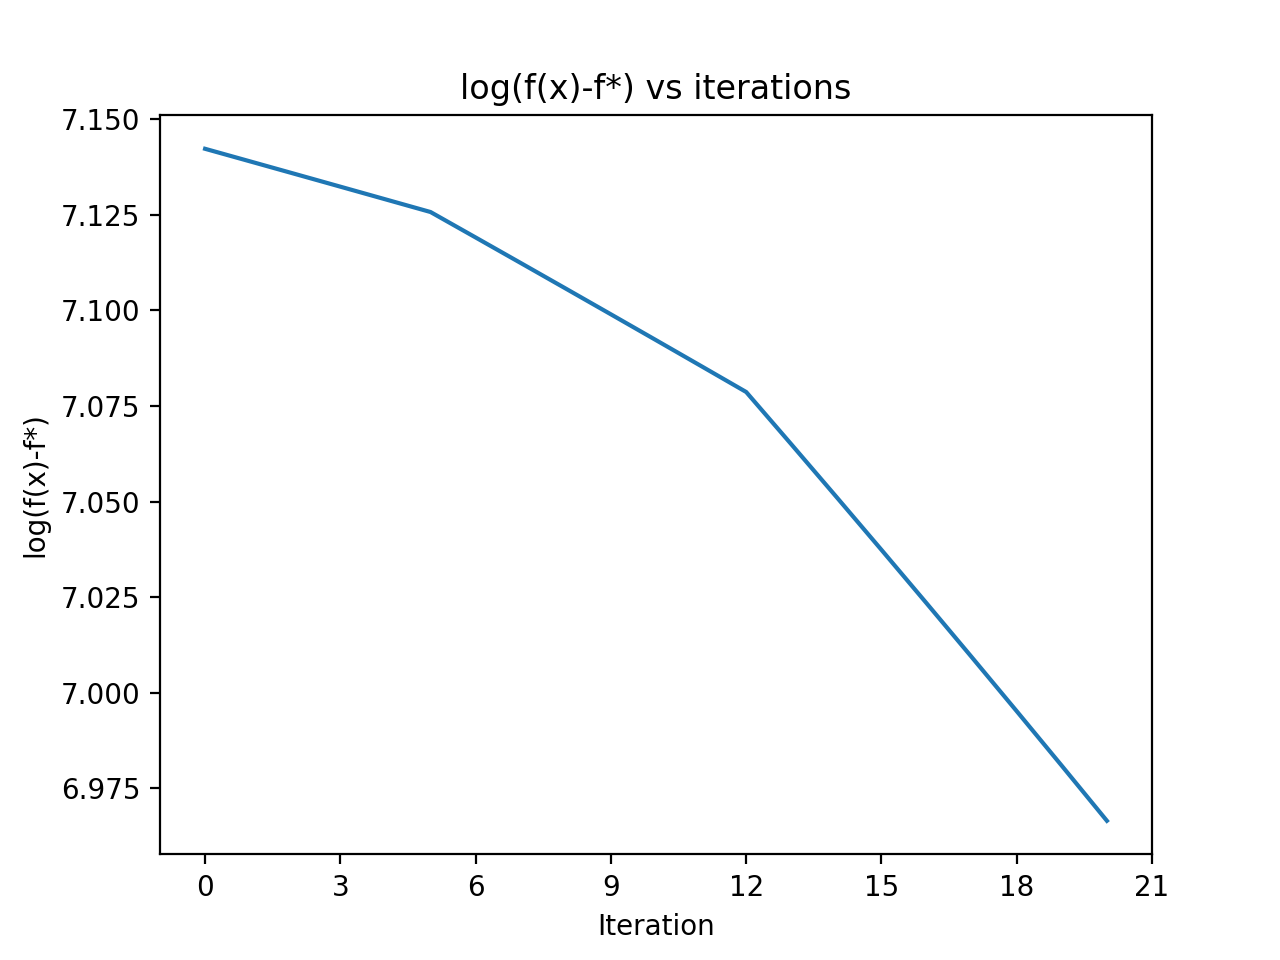
\includegraphics[width=\textwidth]{images/4bi.png}
      \caption{$\log(f(x) - f^*)$, using confidence region Newton method, $x_0 = 0$}
  \end{minipage}
  \hfill
  \begin{minipage}[b]{0.4\textwidth}
      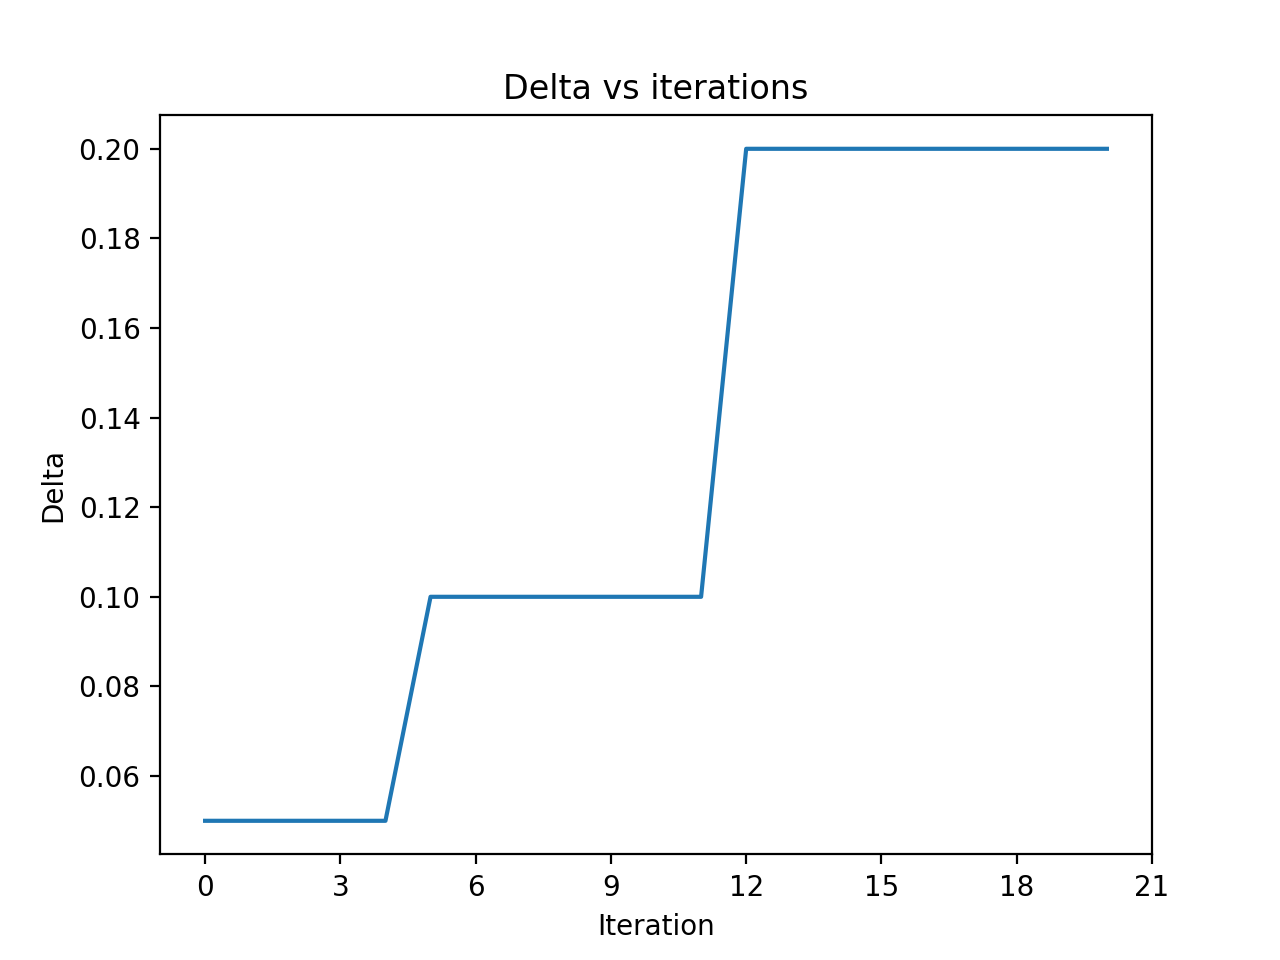
\includegraphics[width=\textwidth]{images/4bii.png}
      \caption{$\Delta_k$, using confidence region Newton method, $x_0 = 0$}
  \end{minipage}

\end{figure}

\hfill \break %SPACE









\begin{enumerate}
  \setcounter{enumi}{2}
  \item Use the accelerated Nesterov method with backtracking.
\end{enumerate}

\paragraph{Solution:}

This method took $3.44$ hours to complete. Python3 code to solve this problem is given by:

\begin{lstlisting}[language=Python]
## Accelerated Nesterov method with backtracking

dots = {}
fs = {}
gradients = {}
time4 = perf_counter()

X = [zeros(n, dtype=float16)] # Initial point x_0 = 0
Fx = [f(X[-1],A)]
lambda_prev = 0
lambda_curr = 1
gamma = 1
y_prev = X[-1]
alpha = 0.15 # Initial alpha
GRADIENTS = [gradient(X[-1], A)] # Initial gradient

iterations = 0

while (norm(GRADIENTS[-1]) > epsilon) and (iterations < max_iterations):
    print("Iteration", iterations)
    print("f(x_k):", Fx[-1])
    print("x_k:", X[-1]) 

    iterations += 1
    sub_iterations = 0

    y_curr = X[-1] - alpha * GRADIENTS[-1]
    X.append((ONE - gamma) * y_curr + gamma * y_prev)
    y_prev = y_curr

    lambda_tmp = lambda_curr
    lambda_curr = (1 + sqrt(1 + 4 * lambda_prev * lambda_prev)) / 2
    lambda_prev = lambda_tmp

    gamma = (1 - lambda_prev) / lambda_curr

    Fx.append(f(X[-1], A))
    GRADIENTS.append(gradient(X[-1], A))

time5 = perf_counter()

print("Accelerated Nesterov method with backtracking completed")
print("Iterations:", iterations)
print("Total time elapsed:", (time5 - time4)/3600, "hours")

log_Fx = [log(f - f_optimal) for f in Fx]
graph(range(iterations+1), log_Fx, "log(f(x)-f*) vs iterations", "Iteration", "log(f(x)-f*)", "4ci")
\end{lstlisting}

\begin{figure}[!tbp]
  \centering
  \begin{minipage}[b]{0.4\textwidth}
      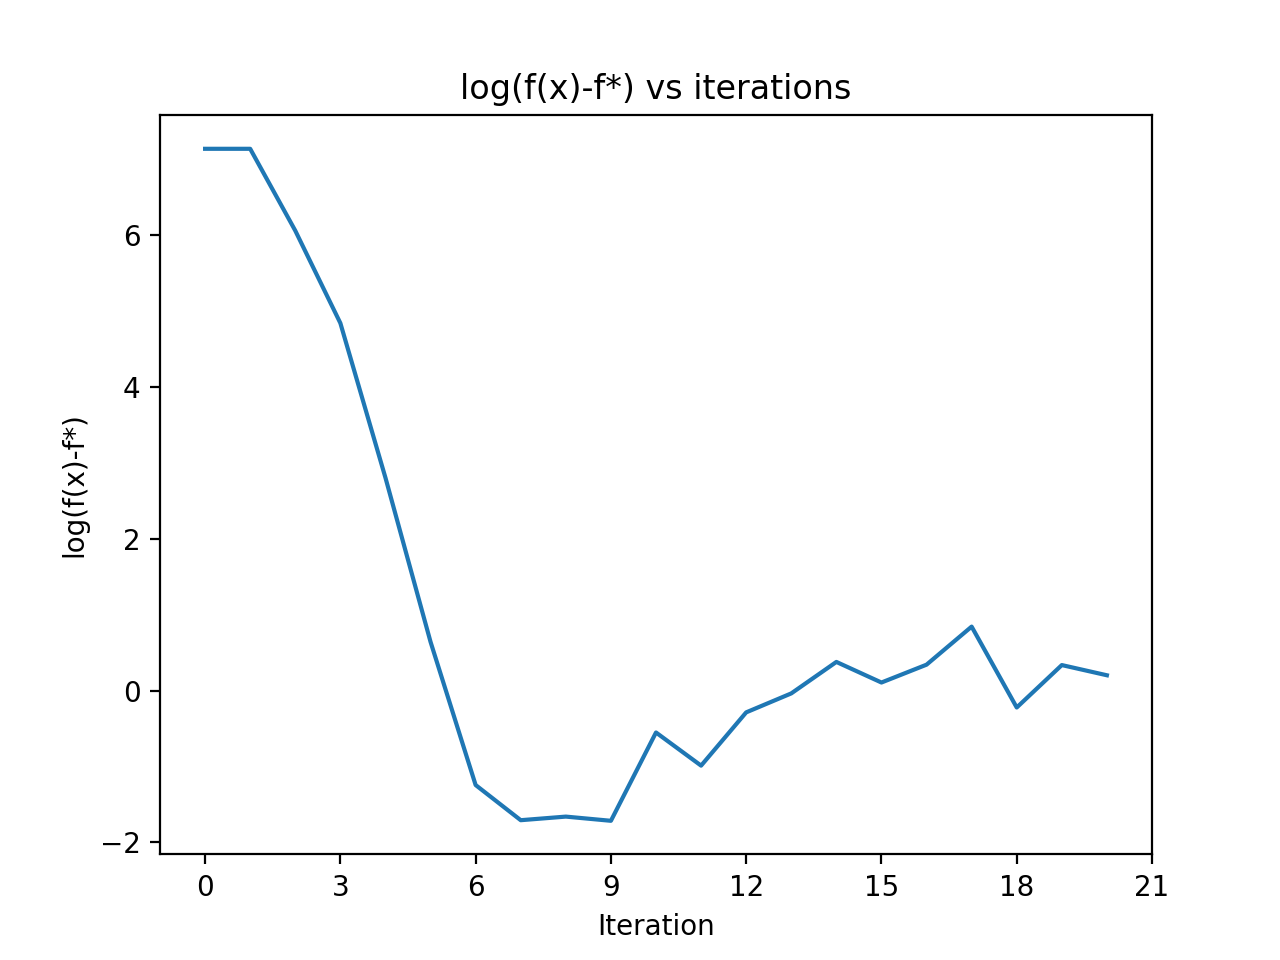
\includegraphics[width=\textwidth]{images/4ci.png}
      \caption{$\log(f(x) - f^*)$, using accelerated Nesterov method, $x_0 = 0$}
  \end{minipage}
\end{figure}




\hfill \break %SPACE

\begin{enumerate}
  \setcounter{enumi}{3}
  \item Use the stochastic gradient method with \textit{mini-batch}, that is, in each iteration choose only some terms in the sums to calculate the gradient, the number of terms chosen is the \textit{mini-batch}. Change the \textit{mini-batch} size and compare.

\end{enumerate}

\paragraph{Solution:}


Here the mini-batch sizes are $500, 200 \text{ and } 100$. They took 
$0.91$, $0.36$ and $0.18$ hours to complete respectively. But in all cases, 
the method made the function get out of its domain. Python3 code to solve this problem is given by:

\begin{lstlisting}[language=Python]
  ## Stochastic gradient descent with mini-batches of size m/4, m/10, m/20

  def stochastic_gradient(x, A, batch):
      result = ones(n)
      with Bar('Gradient', fill='#', suffix='%(percent).1f%% - %(eta)ds', max=n) as bar:
          for i in range(n):
              for j in batch:
                  result[i] += A[j][i] / (ONE - optimized_dot(A[j],x))
              result[i] += TWO * x[i] / (ONE - x[i]*x[i])
              bar.next()
      return result
  
  def stochastic_gradient_method(batch_size):
      time_a = perf_counter()
      alpha = 0.15 # Initial alpha
      X = [zeros(n, dtype=float16)] # Initial point x_0 = 0
      Fx = [f(X[-1],A)]
      batch = sample(range(m), batch_size)
      batch.sort()
      STOCHASTIC_GRADIENTS = [stochastic_gradient(X[-1], A, batch)] # Initial gradient
      iterations = 0
      while (norm(STOCHASTIC_GRADIENTS[-1]) > epsilon) and (iterations < max_iterations):
          print("Iteration", iterations)
          print("f(x_k):", Fx[-1])
          print("x_k:", X[-1])
          print("Batch size:", batch_size)
          iterations += 1
          X.append(X[-1] - alpha * STOCHASTIC_GRADIENTS[-1])
          Fx.append(f(X[-1], A))
          batch = sample(range(m), batch_size)
          batch.sort()
          STOCHASTIC_GRADIENTS.append(stochastic_gradient(X[-1], A, batch))
      time_b = perf_counter()
      print("Stochastic gradient method with batch size", batch_size, "completed")
      print("Iterations:", iterations)
      print("Total time elapsed:", (time_b - time_a)/3600, "hours")
      return Fx
  
  dots = {}
  fs = {}
  batch_size = m//4 # Size of the mini-batches
  Fx = stochastic_gradient_method(batch_size)
  log_Fx = [log(f - f_optimal) for f in Fx]
  graph(range(iterations+1), log_Fx, "log(f(x)-f*) vs iterations", "Iteration", "log(f(x)-f*)", "4di")
  
  dots = {}
  fs = {}
  batch_size = m//10 # Size of the mini-batches
  Fx = stochastic_gradient_method(batch_size)
  log_Fx = [log(f - f_optimal) for f in Fx]
  graph(range(iterations+1), log_Fx, "log(f(x)-f*) vs iterations", "Iteration", "log(f(x)-f*)", "4dii")
  
  dots = {}
  fs = {}
  batch_size = m//20 # Size of the mini-batches
  Fx = stochastic_gradient_method(batch_size)
  log_Fx = [log(f - f_optimal) for f in Fx]
  graph(range(iterations+1), log_Fx, "log(f(x)-f*) vs iterations", "Iteration", "log(f(x)-f*)", "4diii")
\end{lstlisting}

\begin{figure}[!tbp]
  \centering
  \begin{minipage}{0.45\textwidth}
    \centering
    
\includegraphics[width=\textwidth]{Polyak_vs_Iterations.png}
    \caption{Polyak vs Iterations}
    \label{fig:3}
  \end{minipage}
  \hfill
  \begin{minipage}{0.45\textwidth}
    \centering
    
\includegraphics[width=\textwidth]{Stochastic_subgradient_vs_Iterations.png}
    \caption{Stochastic subgradient vs Iterations}
    \label{fig:4}
  \end{minipage}
\end{figure}




\end{document}